%% rnaastex.cls is the classfile used for Research Notes. It is derived
%% from aastex61.cls with a few tweaks to allow for the unique format required.
%% (10/15/17)
%%\documentclass{rnaastex}

%% Better is to use the "RNAAS" style option in AASTeX v6.2
%% (01/08/18)
\documentclass[RNAAS]{aastex62}

%% Define new commands here
\newcommand\latex{La\TeX}
\newcommand{\rsol}{R_{\odot}}
\newcommand{\lsol}{L_{\odot}}
\newcommand{\msol}{M_{\odot}}
\newcommand{\mearth}{M_{\oplus}}
\newcommand{\rearth}{R_{\oplus}}
\newcommand{\mjup}{M_{\rm Jup}}
\newcommand{\rjup}{R_{\rm Jup}}

\begin{document}

\title{taktent - a Python package for simulating and testing SETI strategies}

%% Note that the corresponding author command and emails has to come
%% before everything else. Also place all the emails in the \email
%% command instead of using multiple \email calls.
\correspondingauthor{Duncan Forgan}
\email{dh4gan@gmail.com}

\author[0000-0003-1175-4388]{Duncan Forgan}
\affiliation{Centre for Exoplanet Science, SUPA, University of St Andrews, North Haugh, St Andrews, KY16 9SS, UK}


%% Note that RNAAS manuscripts DO NOT have abstracts.
%% See the online documentation for the full list of available subject
%% keywords and the rules for their use.
\keywords{+++}

%% Start the main body of the article. If no sections in the 
%% research note leave the \section call blank to make the title.

\section{Motivation}

The Search for Extraterrestrial Intelligence (SETI) in our Galaxy is fraught with challenges, even if the Milky Way is replete with technosignatures.  Civilisations choosing to send electromagnetic transmissions must make a series of choices - frequency, bandwidth, direction, beam solid angle, polarisation, etc.  They must also choose whether to send continuous transmissions or pulses.  If pulses are sent, the duration of the pulse, and the time interval between pulses must also be selected.  Finally, if transmissions are to contain information, the transmission must be modulated in some fashion - the choices available for signal modulation are numerous (see e.g. \citealt{Messerschmitt2013,Messerschmitt2015}).  

These choices require SETI searches to explore a parameter space of very high volume and dimensionality - often referred to as ``the cosmic haystack'' \citep{TarterPlanetsLife2007,Wright2018a}.  The size of this haystack motivates the Messaging Extraterrestrial Intelligence (METI) community, who argue that the only means to collapse the haystack to a manageable size is for humans to send transmissions of their own, allowing potential alien interlocutors a better chance of constructing an appropriate signal for us to receive (see e.g. +++, +++ and +++).

SETI surveys are enjoying a revival thanks to private funding efforts such as the Breakthrough Listen initiative \citep{Isaacson2017}.  The astrophysics community's attitude towards SETI science continues to warm, as evidenced by the recent NASA Technosignatures workshop (and accompanying report, \citealt{Participants2018}).   With this new goodwill towards SETI, and the continuing advances in breadth and depth of SETI searches (+++), it is important to motivate underlying observational strategy, and to demonstrate the fraction of the cosmic haystack to which a given search is sensitive.  

Equally, as new forms of technosignature are characterised and modelled, opportunities grow for all-sky astronomical surveys to yield serendipitous detections.  As these surveys are not explicitly designed to capture technosignatures, there is a clear need for tools to characterise their potential yield.  For example, exoplanet transit surveys have the potential to recover several kinds of surface and atmospheric technosignatures \citep[e.g.][]{Lin2014,Korpela2015,Lingam2017a}, as well as signatures of orbital developments and installations \citep[e.g.][]{Socas-Navarro2018}.

In this Note, I introduce a new Python package, \textsc{taktent}(+++)\footnote{The name ``taktent'' is derived from the Scots phrase ``tak tent o' the sma things'', which translates into English as ``pay attention to the little things''.}, to the SETI community.  It allows the user to set up and run agent-based simulations of civilisations engaging in either SETI (observing) or METI (broadcasting).  I will briefly describe the package, and give an example of its use.  The source code is available at \url{github.com/dh4gan/taktent}, and can be installed using the \texttt{pip} package installer (see the github repository for further details).

\section{About the Package}

\noindent \textsc{taktent} is written entirely in object-oriented Python 3.6, using \textsc{numpy} 1.14.3 \citep{Oliphant2006} and \textsc{matplotlib} 2.2.2 \citep{Hunter2007}, and hence requires these for basic operation\footnote{Some additional, optional functionality also requires \texttt{mpl\_toolkits.basemap}}.  The package describes several classes of object that drive the agent-based simulation of the SETI problem.  The \texttt{Agent} base class is extended into two subclasses - \texttt{Observer} and \texttt{Transmitter} - which represent an observing and transmitting civilisation, respectively.  Both classes possess a spatial location\footnote{Simulations are conducted in Cartesian co-ordinates, and are mediated by a bespoke \texttt{Vector3D} class} (which includes the possibility of being in orbit around a host star), as well as a pointing vector (for either listening or broadcasting), with a defined opening angle.  This defines a \texttt{Transmitter}'s beam size, and an \texttt{Observer'}s field of view.

\texttt{Observers} possess a range of frequencies which they can listen at, as well as a sensitivity limit (defined as a minimum observable flux per unit frequency).  \texttt{Transmitters} emit radiation at a specific frequency, with a defined bandwidth and solid angle.  They also transmit either continuously or in the form of pulses, with a defined duration and interval between pulses.

The direction of both classes' pointing is governed by a \texttt{Strategy} object, which can either be a series of discrete pointing choices (a \texttt{PointingStrategy}), or a smooth scan across the sky (a \texttt{ScanningStrategy}).

The simulation itself is driven by the \texttt{Population} class, which allows the generation of \texttt{Transmitters} and \texttt{Observers}, and conducts observations, recording and plotting detection data where requested.  For several examples of \textsc{taktent} in operation, please see \url{github.com/dh4gan/taktent/examples}.

\textsc{taktent} models the finite travel time of electromagnetic signals, and their inverse square law ($1/r^2$) decay of flux, as well as the Doppler drift due to the relative motion of the Observer and Transmitter.  It should also be noted that the package's construction is flexible enough that if the user wishes to model SETI signals using a different messenger particle or mechanism, this is also achievable.  For example, one can model gravitational waves (which have a $1/r$ flux decay law) by adjusting the Transmitter object's \texttt{decaylaw} parameter, or with slower messenger particles by reducing the \texttt{broadcastspeed} parameter.

\section{A Science Example}

\noindent In this example, I simulate a SETI survey in a galaxy populated by 1000 \texttt{Transmitters} and one \texttt{Observer} residing in the Galactic Habitable Zone \citep{GHZ,Gowanlock2011}.  The zone is defined as an annulus between 6 and 10 kpc, with a surface density of stars that decays as $e^{-R/R_S}$, with the scale length $R_S=3$ kpc. 

Each \texttt{Transmitter} broadcasts isotropically, with frequencies, start times, pulse durations and intervals sampled from uniform distributions.  The \texttt{Observer} object is initialised with a \texttt{scanningStrategy} that sweeps the x-y plane with a period of 10 years.  For the sake of brevity, I do not reproduce all the initial conditions here - the code that defines and runs this simulation can be found in the github repository at \url{github.com/dh4gan/taktent/examples/science\_example.py}.  Four different Monte Carlo Realisations of the simulation are run.

%% An example figure call using \includegraphics
\begin{figure}[h!]
\begin{center}
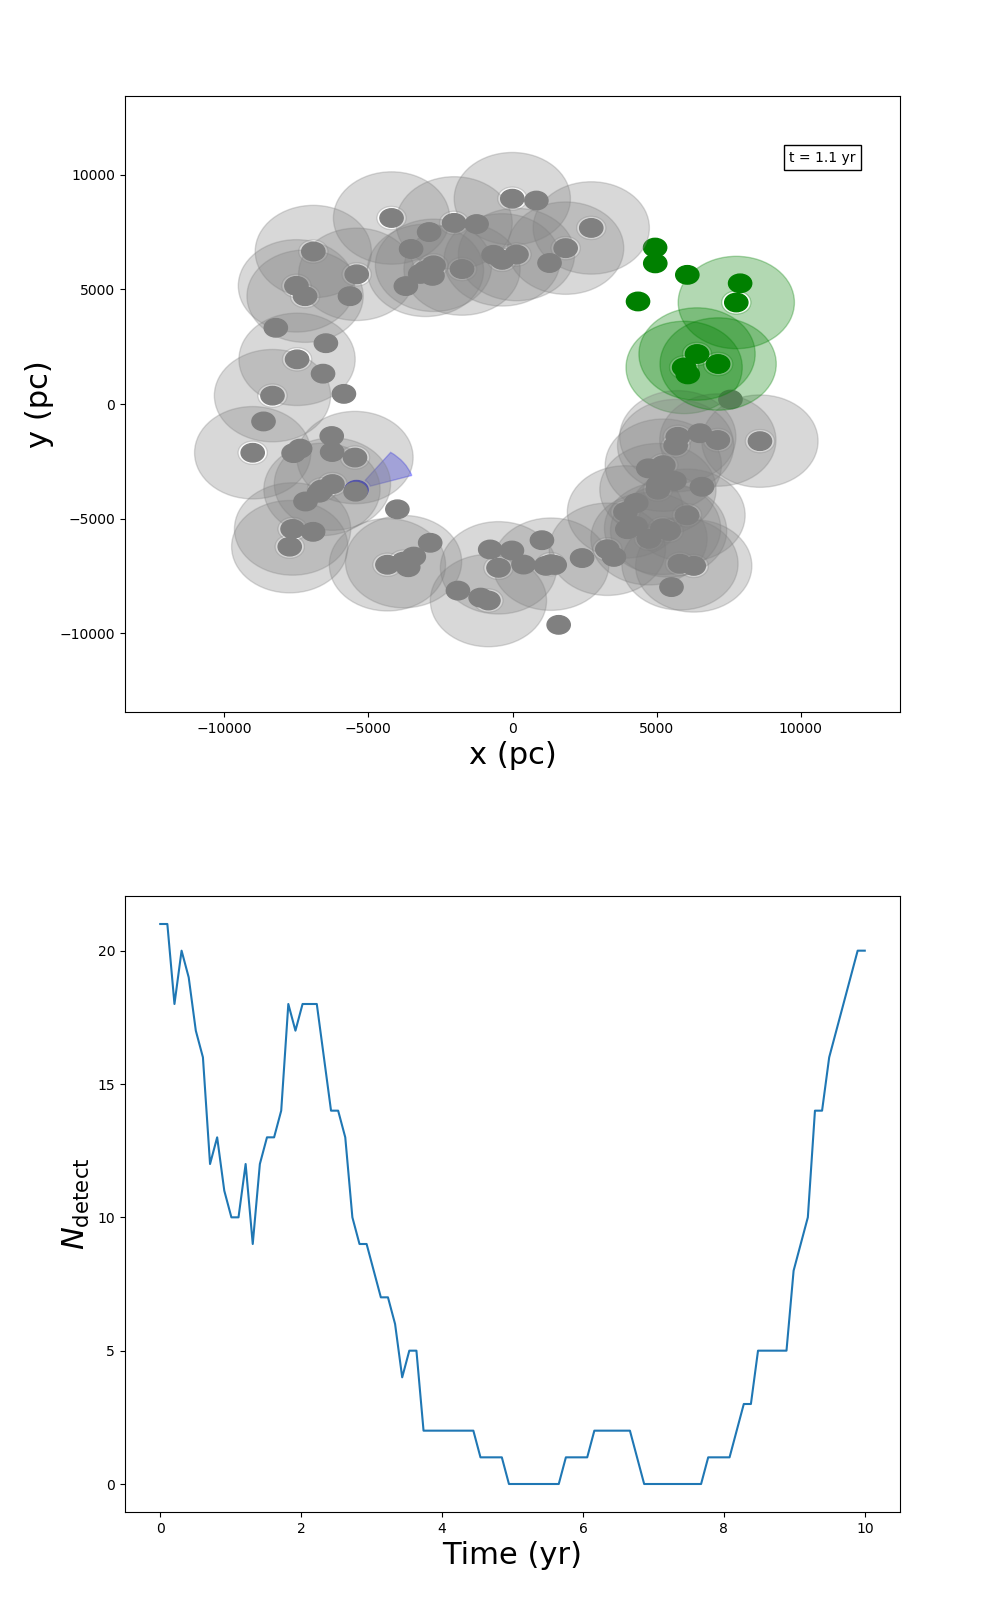
\includegraphics[scale=0.5]{combined.png}
\caption{Top:  A snapshot from one realisation of \textsc{taktent}.  Civilisations are represented as solid dots, with halos/wedges indicating whether the civilisation is actively broadcasting/observing.  The \texttt{Observer} object (blue) resides in the bottom left quadrant, and has detected approximately 10 \texttt{Transmitters} (colored green) in its field of view.  Note that some \texttt{Transmitters} are not active at this time, but are still observable due to delay caused by the finite travel time of the transmission. Bottom: The number of \texttt{Transmitters} detected by the \texttt{Observer} as a function of time. \label{fig:1}}
\end{center}
\end{figure}


The top panel of Figure \ref{fig:1} shows a snapshot from the simulation, where the \texttt{Observer} object is able to detect 11 \texttt{Transmitter}s at that instant.  In the bottom panel of Figure \ref{fig:1}, I show the number of detections achieved by the \texttt{Observer} object as a function of time for a single realisation.  

The \texttt{Population} object also records aggregated data from the simulation (mean distance from an \texttt{Observer} to a detected \texttt{Transmitter}, mean pulse duration of detected \texttt{Transmitter}s, and so on), while each \texttt{Observer} and \texttt{Transmitter} can write all detections at any timestep to file.  A key avenue for future development of \textsc{taktent} is determining what data/metrics should be outputted to file, which will depend on the desires of its future userbase.

\section{Conclusion}

\noindent I will unfortunately not be able to use this package to produce science, as I am leaving academia.  For this reason, I have published this code open-source in the hope it is used to improve and refine SETI observational strategies.  I welcome contributions from those wishing to develop the code further - please see the \texttt{CONTRIBUTING.md} file at \url{github.com/dh4gan/taktent} for more details.

%% An example figure call using \includegraphics
%\begin{figure}[h!]
%\begin{center}
%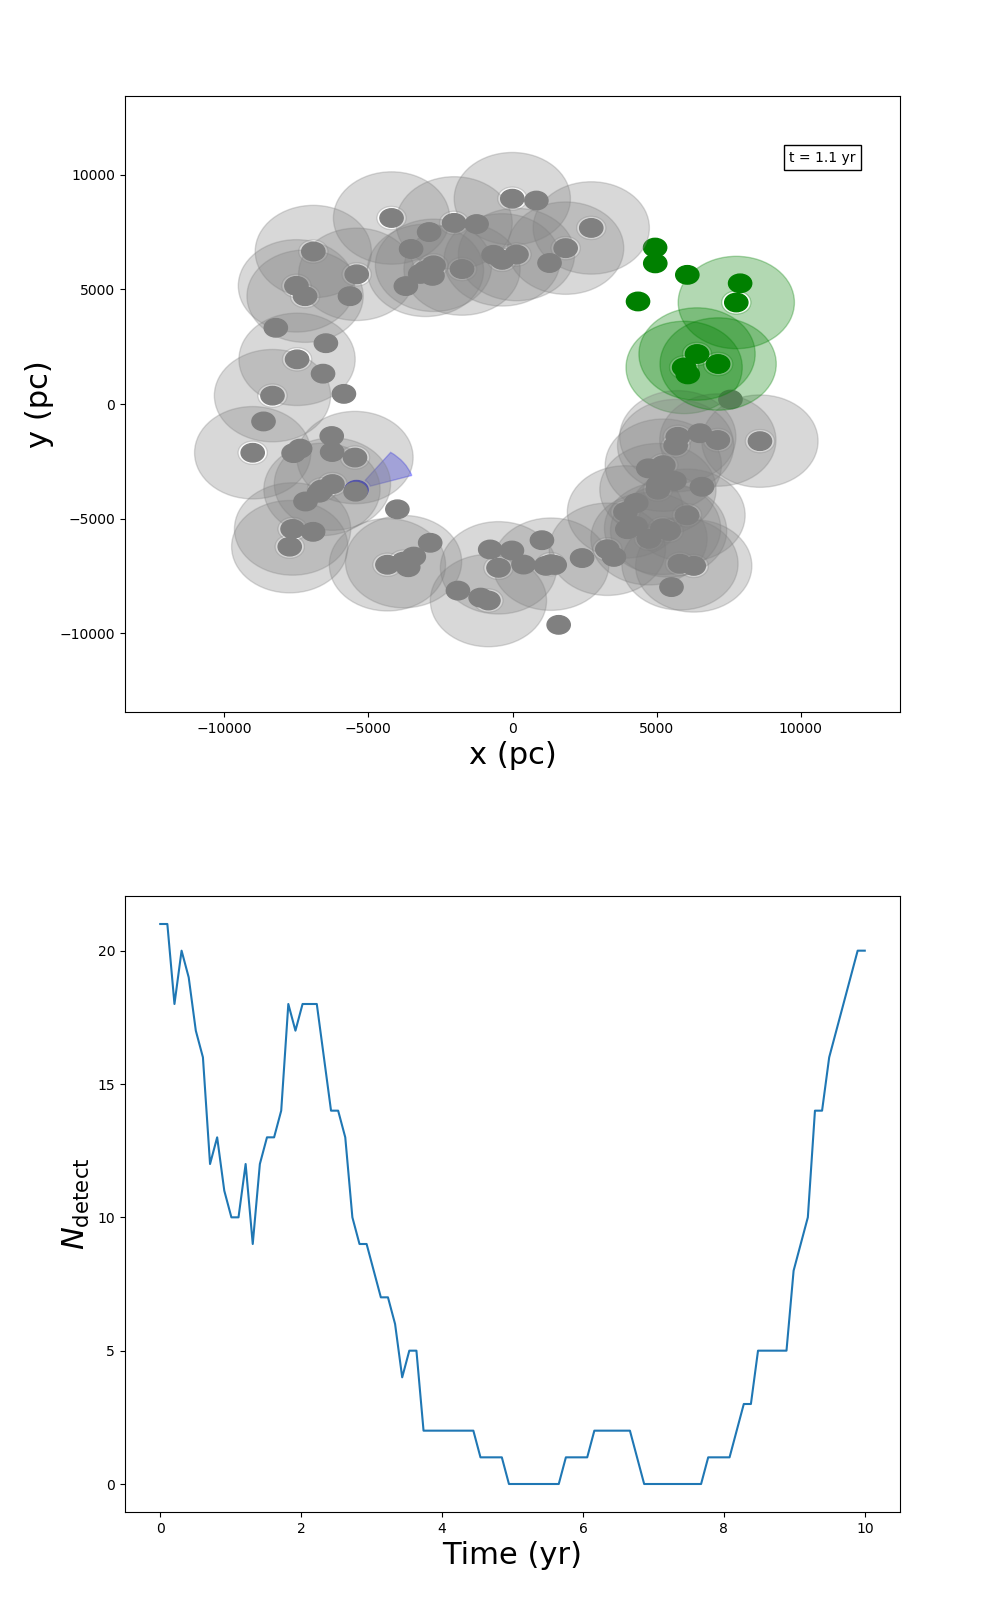
\includegraphics[scale=0.7]{combined.png}
%\caption{Top: The minimum, maximum and mean surface temperature of the moon-moon over a 20 year time interval.  Note that this curve has been downsampled to show temperature fluctuations over the planetary period.  Bottom: The mean temperature over a 1 year time interval.  This has not been downsampled, and reflects the variations on the exomoon candidate's period of 0.03 years. \label{fig:1}}
%\end{center}
%\end{figure}

%% An example table using AASTeX's deluxetable. Note that since
%% only one figure OR one table is allowed this is commented out.
%\begin{deluxetable}{ccl}
%\tablecaption{Example table some English and Greek letters\label{tab:1}}
%\tablehead{
%\colhead{Index number} & \colhead{English} & \colhead{Greek}
%}
%\startdata
%1 & a & alpha ($\alpha$) \\
%2 & b & beta ($\beta$) \\
%3 & c & gamma ($\gamma$) \\
%4 & d & delta ($\delta$) \\
%5 & e & epsilon ($\epsilon$) \\
%\enddata
%\tablecomments{Long tables should only show a short example with the full
%version as a machine readable table with the article.}
%\end{deluxetable}  

\acknowledgments

\bibliographystyle{mnras}
\bibliography{taktent}


\end{document}
